% orbit-recovery.tex — \input'd from thesis/experiments.tex
%
% Sources: experiments/orbit-recovery/orbit-recovery.jsonl (112 records),
%   experiments/orbit-recovery/orbit_recovery.py (analysis script),
%   experiments/orbit-recovery/README.md (findings).
%
% Structure:
%   - Setup: what we validate, dataset, metrics, thresholds
%   - Results: per-F error table, 112/112 pass
%   - Solution dimension: distribution, geometric interpretation

\subsection{Orbit Recovery Validation}
\label{sec:orbit-recovery}

The EHZ algorithm (Algorithm~\ref{alg:ehz}) outputs a facet sequence~$S$
and weights~$\beta$. Base point recovery
(Lemma~\ref{lem:base-point-recovery}) reconstructs the starting
point~$b = \gamma(0)$ of the corresponding Reeb orbit on~$\partial K$.
This experiment validates that the recovered orbit is geometrically
consistent: it closes up, stays on~$\partial K$, and has the correct
action.

\subsubsection*{Setup}

We test on 112~polytopes: 7~known polytopes from the literature
(Table~\ref{tab:literature-polytopes}) and 105~random polytopes
(20~each for $F = 5, \ldots, 8$, 15~for $F = 9$, 10~for $F = 10$).
For each polytope, we compute the capacity, recover the base
point~$b$, reconstruct the orbit~$\gamma$, and measure four error
metrics:
\begin{itemize}
  \item \textbf{Closure error}: $\lVert \gamma(T) - \gamma(0) \rVert$,
    where $T$~is the period.
  \item \textbf{On-facet error}: maximum distance of any breakpoint
    from its assigned facet.
  \item \textbf{Inequality violation}: maximum violation of
    $\langle n_i, \gamma(t_j) \rangle \le h_i$ across all facets~$i$
    and breakpoints~$t_j$.
  \item \textbf{Action error}: $\lvert A(\gamma) - c_{\mathrm{EHZ}}(K) \rvert$,
    where~$A(\gamma)$ is the symplectic action of the recovered orbit.
\end{itemize}
Validation thresholds are $10^{-6}$ for the three geometric metrics and
$10^{-5}$ for action error (which accumulates rounding over the full
orbit).

\subsubsection*{Results}

All 112~polytopes pass validation.
Table~\ref{tab:orbit-recovery-errors} shows maximum errors by facet
count. Known polytopes achieve errors near machine epsilon (${\sim}10^{-15}$).
Random polytopes have errors below~$10^{-8}$ for $F \le 9$; at
$F = 10$, accumulated floating-point error in the KKT solve and orbit
reconstruction raises the maximum action error to~$1.83 \times 10^{-6}$,
still well within the $10^{-5}$~threshold.

\begin{table}[h]
\centering
\small
\begin{tabular}{rrrrrr}
\toprule
$F$ & $N$ & Closure & On-facet & Violation & Action \\
\midrule
\multicolumn{6}{l}{\emph{Known polytopes (all $F$)}} \\
 & 7 & $2.2 \times 10^{-15}$ & $1.4 \times 10^{-15}$ & $1.3 \times 10^{-15}$ & $5.8 \times 10^{-15}$ \\
\midrule
\multicolumn{6}{l}{\emph{Random polytopes (by $F$)}} \\
5 & 20 & $1.1 \times 10^{-9}$ & $3.1 \times 10^{-10}$ & $3.1 \times 10^{-10}$ & $4.4 \times 10^{-9}$ \\
6 & 20 & $8.5 \times 10^{-11}$ & $5.5 \times 10^{-12}$ & $2.0 \times 10^{-11}$ & $4.5 \times 10^{-11}$ \\
7 & 20 & $2.5 \times 10^{-11}$ & $5.4 \times 10^{-12}$ & $1.5 \times 10^{-11}$ & $3.7 \times 10^{-11}$ \\
8 & 20 & $6.7 \times 10^{-11}$ & $1.7 \times 10^{-11}$ & $1.7 \times 10^{-11}$ & $1.2 \times 10^{-10}$ \\
9 & 15 & $1.7 \times 10^{-10}$ & $3.1 \times 10^{-11}$ & $6.5 \times 10^{-12}$ & $1.6 \times 10^{-10}$ \\
10 & 10 & $3.7 \times 10^{-7}$ & $6.8 \times 10^{-8}$ & $6.8 \times 10^{-8}$ & $1.8 \times 10^{-6}$ \\
\bottomrule
\end{tabular}
\caption{Maximum error metrics for orbit recovery, by facet count.
  Errors stay near machine epsilon for $F \le 9$ and remain within
  validation thresholds at $F = 10$.}
\label{tab:orbit-recovery-errors}
\end{table}

Figure~\ref{fig:orbit-recovery-errors} shows the error scaling across
facet counts. The jump at $F = 10$ likely reflects accumulated floating-point
error in the KKT solve and orbit reconstruction for higher-dimensional
linear programs.

\begin{figure}[h]
\centering
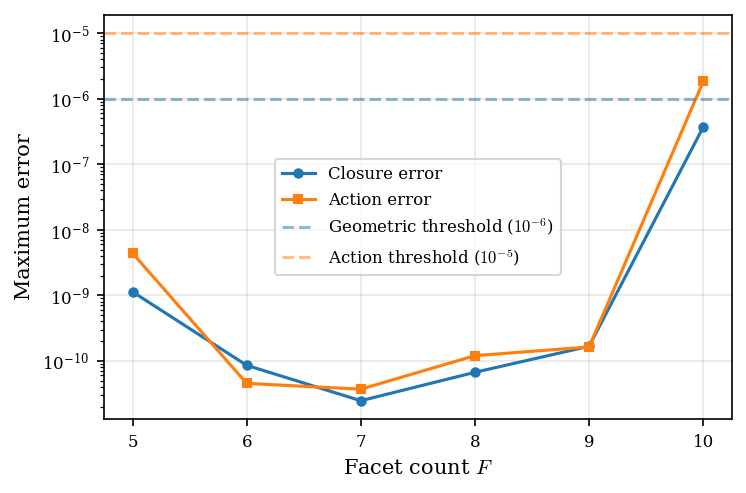
\includegraphics{../experiments/orbit-recovery/orbit_recovery_errors.png}
\caption{Maximum closure and action error by facet count (random
  polytopes only). Both metrics remain well below their validation
  thresholds (dashed lines).}
\label{fig:orbit-recovery-errors}
\end{figure}

\subsubsection*{Solution Dimension}

Base point recovery solves the linear system~$N_S b = r$, where~$N_S$
collects the outward normals of the active facets. The solution
dimension is $\dim = 4 - \operatorname{rank}(N_S)$: when the active
normals are linearly independent, the base point is unique.

Of the 112~polytopes, 108 ($96.4\%$) have a unique base point
($\dim = 0$). The four exceptions are all known polytopes with
special structure: the hypercube ($\dim = 2$, 4~active facets),
both symplectic products ($\dim = 2$, 3--4~active facets), and the
Lagrangian triangle--square product ($\dim = 1$, 5~active facets).
In each case, the active normals are linearly dependent due to the
product structure. No random polytope exhibits non-uniqueness,
consistent with this being a measure-zero condition.

For further numerical error analysis, see Appendix~\ref{app:numerical}.
